\section{采集}

采集节点只有一个，选项很多。选平台，选采集内容，填目标数量，选格式，剩下的交给程序。
平台之间的差别收在一张表里，面板只显示这个平台真正支持的那几项。

\begin{table}[H]\centering
\caption{各平台能采集的内容}
\label{tab:platforms}
\small
\begin{tabularx}{\textwidth}{p{2.6cm}X}
\toprule
平台 & 可选内容 \\
\midrule
知乎 & 关键词帖子与文章、某作者的作品、热榜、评论 \\
微博 & 关键词帖子、某作者的作品、热搜、评论 \\
小红书 & 关键词笔记、某作者的笔记、评论 \\
微信公众号 & 关键词文章正文 \\
哔哩哔哩 & 关键词视频、某作者的作品、热榜、评论 \\
抖音 & 某作者的作品、热榜、评论 \\
红果短剧 & 四个榜单、评论（仅 Windows 桌面） \\
中国知网 & 文献检索结果，按篇数导出 \\
YouTube & 关键词视频、频道作品、评论 \\
X & 关键词帖子、某作者的作品、评论 \\
Instagram & 只能保存登录状态，采集未接入 \\
\bottomrule
\end{tabularx}
\end{table}

采集引擎有两套。一套是浏览器，用 Selenium 驱动本机 Chrome；另一套是 CatBus，一个独立的外部采集器，
走自己的适配器与账号文件。两套后端能采什么、输出哪些列，都读各自的清单，选到不支持的组合会置灰并写明原因。

浏览器这套要登录状态。一个平台一个账号对应一份 Cookie 快照加一个独立的浏览器目录，对站点来说就是一台连续的设备。
默认那份登录也有名字，叫默认账号。采集节点的账号下拉列出当前存了登录的账号。

按下执行前会做一次登录预检：用这次真要用的浏览器打开平台首页，看它还认不认这份登录。跳到登录页就拦下来并点名平台。
因为网络慢、验证码、站点忙而没法判断的情况不拦，只记一笔，让你自己决定。预检可以关，关掉后由采集自己撞墙再报错。

采集支持分批落库。节点里填分片大小，每满 N 行先写一个带编号的文件，运行中就能打开看，结束时合成一份。
分片文件名可以带采集时间或者本次创建时间，跑第二遍不覆盖第一遍。

采集也支持上游喂任务。上游是一张表时，在节点里指定一列，程序逐行取这一列的链接或名字去采。
这是批量补抓评论最省事的做法，热榜转评论那一节会完整走一遍。

采集结束时报一个数。站点提前到底就按站点自己的话结束，并说明第几页到底；没到目标数量就停下时，控制台写清为什么停，
不会把短表当成长表交给你。

\section{保存登录}

要采带登录态的内容，先存一份登录，存一次以后一直用。

\begin{enumerate}
\item 菜单条点“\texttt{Cookies}”，打开登录设置。左边选平台，右边是这一份登录的字段。
\item “\texttt{账号}”留空就是默认账号，填一个新名字则另存一份，用来对付限流或换号。
\item 点“\texttt{浏览器生成}”，程序弹出一个 Chrome 窗口，你在里面扫码或输密码登录，登录完回到本面板点“\texttt{已完成登录}”，Cookie 自动收下来。
\item 也可以把浏览器导出的 Cookie JSON 粘进大框，点“\texttt{保存 Cookies}”。
\item 点“\texttt{验证 Cookie}”，程序打开平台首页问一句还认不认，认就写可用，不认就写失效。
\end{enumerate}

\begin{figure}[H]\centering
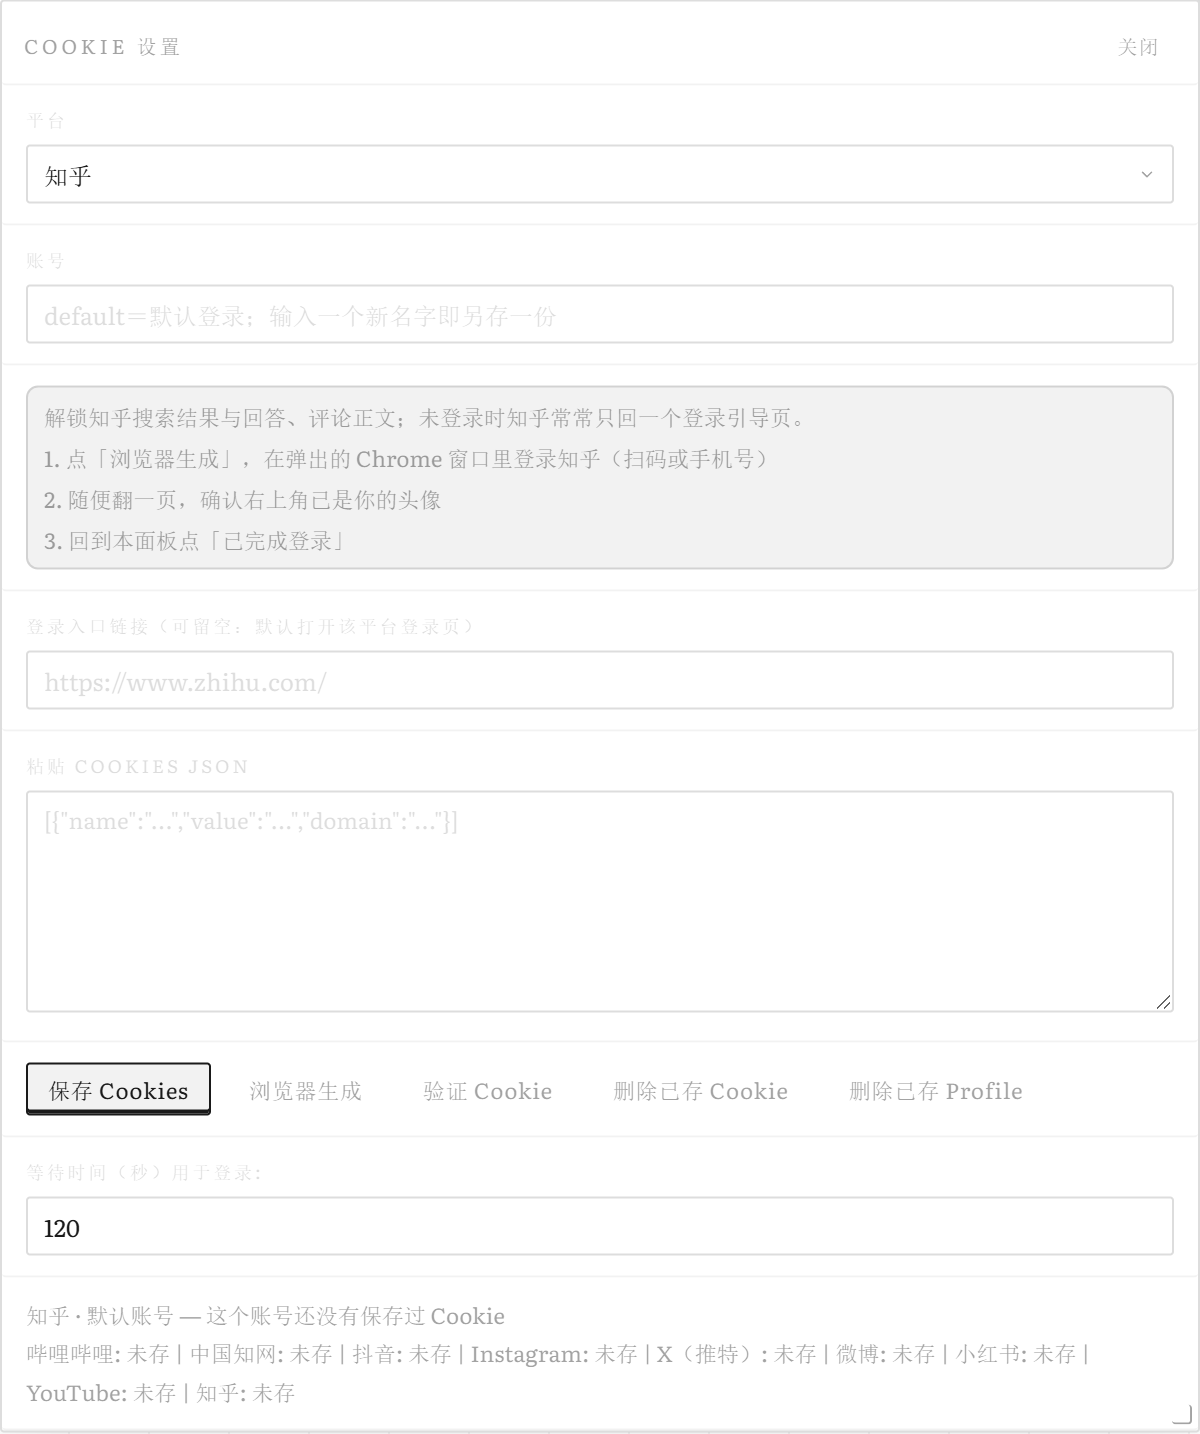
\includegraphics[width=0.56\textwidth]{cookie-dialog.png}
\caption{登录设置：平台、账号、登录入口、粘贴区与四个操作按钮}
\label{fig:cookie-dialog}
\end{figure}

面板底部一行是各平台当前账号的状态，未存、可用、失效一眼可见。存好的登录出现在底部“\texttt{已保存的登录}”表里，
一行一个平台加账号，写着条数与存入时间，每行能重命名、删 Cookie、删浏览器目录。

\begin{figure}[H]\centering
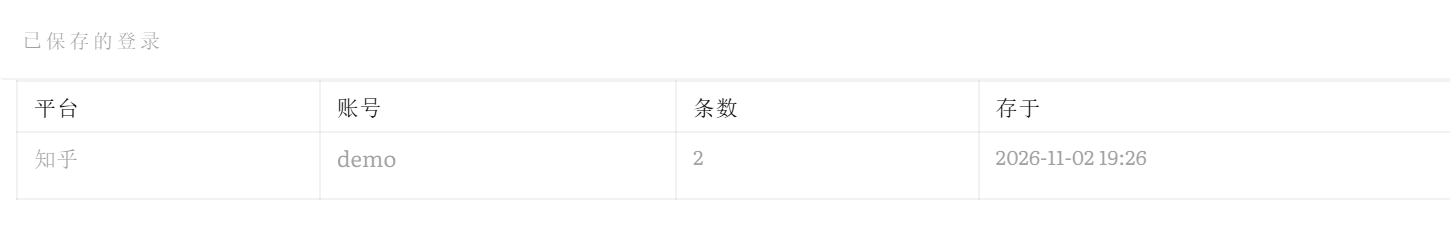
\includegraphics[width=0.86\textwidth]{cookies.png}
\caption{已保存的登录，一行一个平台加账号}
\label{fig:cookies}
\end{figure}

两个删除不一样。删 Cookie 只删那份快照，浏览器目录里的登录态还在，下次采集仍可能是登录的；删 Profile 才是把那台设备登出。
写论文前如果换过账号，两个都要清，免得采到上一个账号的视角。

采集节点里的“\texttt{登录账号}”就是这张表里的名字。选了哪份就用哪份，预检也会用它打开首页核对一遍。

\section{实战一\quad 红果短剧四个热播榜}

这一段从空白画布做出一条能跑的采集链，得到四份 CSV：热播榜、真人剧、AI 剧、漫剧，每个一百条。
红果只能在本机桌面上采，别的系统上这个平台会按名字拒绝。

\subsection{建链}

菜单条点“\texttt{新建}”。节点库拖出“\texttt{工作流命名}”，设置里填“\texttt{红果热播榜}”。
右边放“\texttt{数据源}”，打开设置依次填：

\begin{enumerate}
\item 平台“\texttt{红果短剧}”，采集引擎“\texttt{浏览器}”，采集内容“\texttt{热榜}”。
\item 目标数量 \texttt{100}。这是上限，站点只有五页就写到一百条为止。
\item 榜单选“\texttt{热播榜}”，另外三个是真人剧、AI 剧、漫剧。
\item 重新采集打勾，分片大小填 \texttt{0}，格式 \texttt{CSV}。
\end{enumerate}

右边再放“\texttt{输出}”：操作“\texttt{保存}”，格式 \texttt{CSV}，文件名“\texttt{红果热播榜.csv}”，勾上“\texttt{文件名追加本次运行时间}”。

\begin{figure}[H]\centering
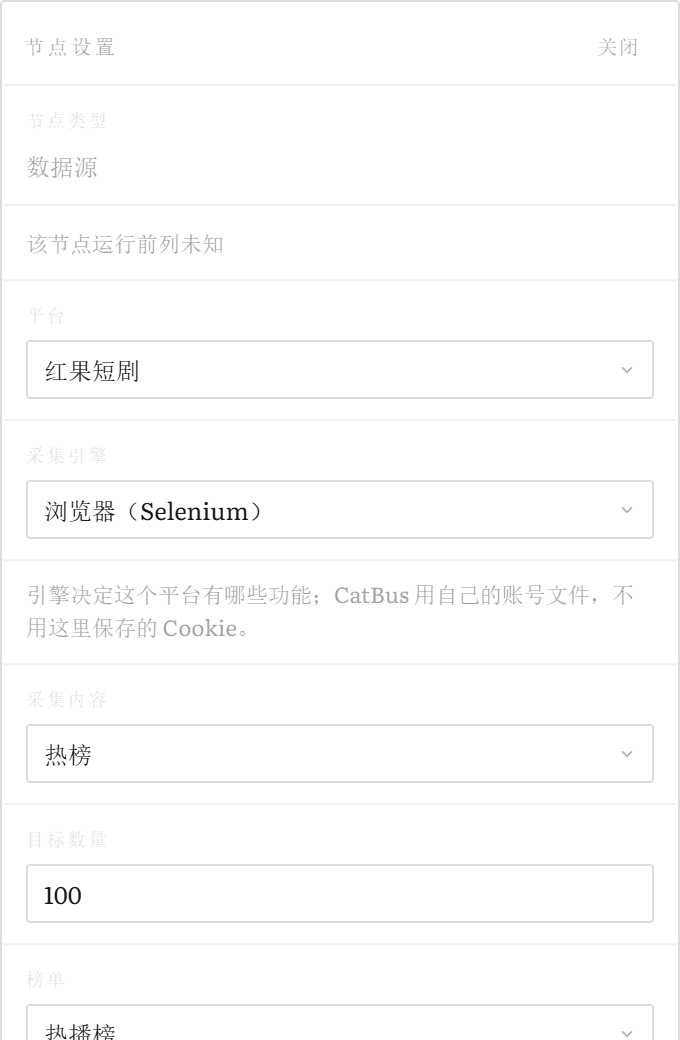
\includegraphics[width=0.31\textwidth]{hg-source.png}
\caption{红果数据源：平台、内容、数量、榜单、重新采集、格式}
\label{fig:hg-source}
\end{figure}

从命名节点右侧圆点拖到数据源左侧，再从数据源拖到输出左侧。两条线一接，这条链就成立。

\subsection{复制成四条}

把三个节点框选，Ctrl 加 C，Ctrl 加 V 三次。每条链改三处：名字、榜单、文件名。
四条链互不相连，摆成四行，画布就是下图。节点上的绿勾是上一次跑完留下的。

\begin{figure}[H]\centering
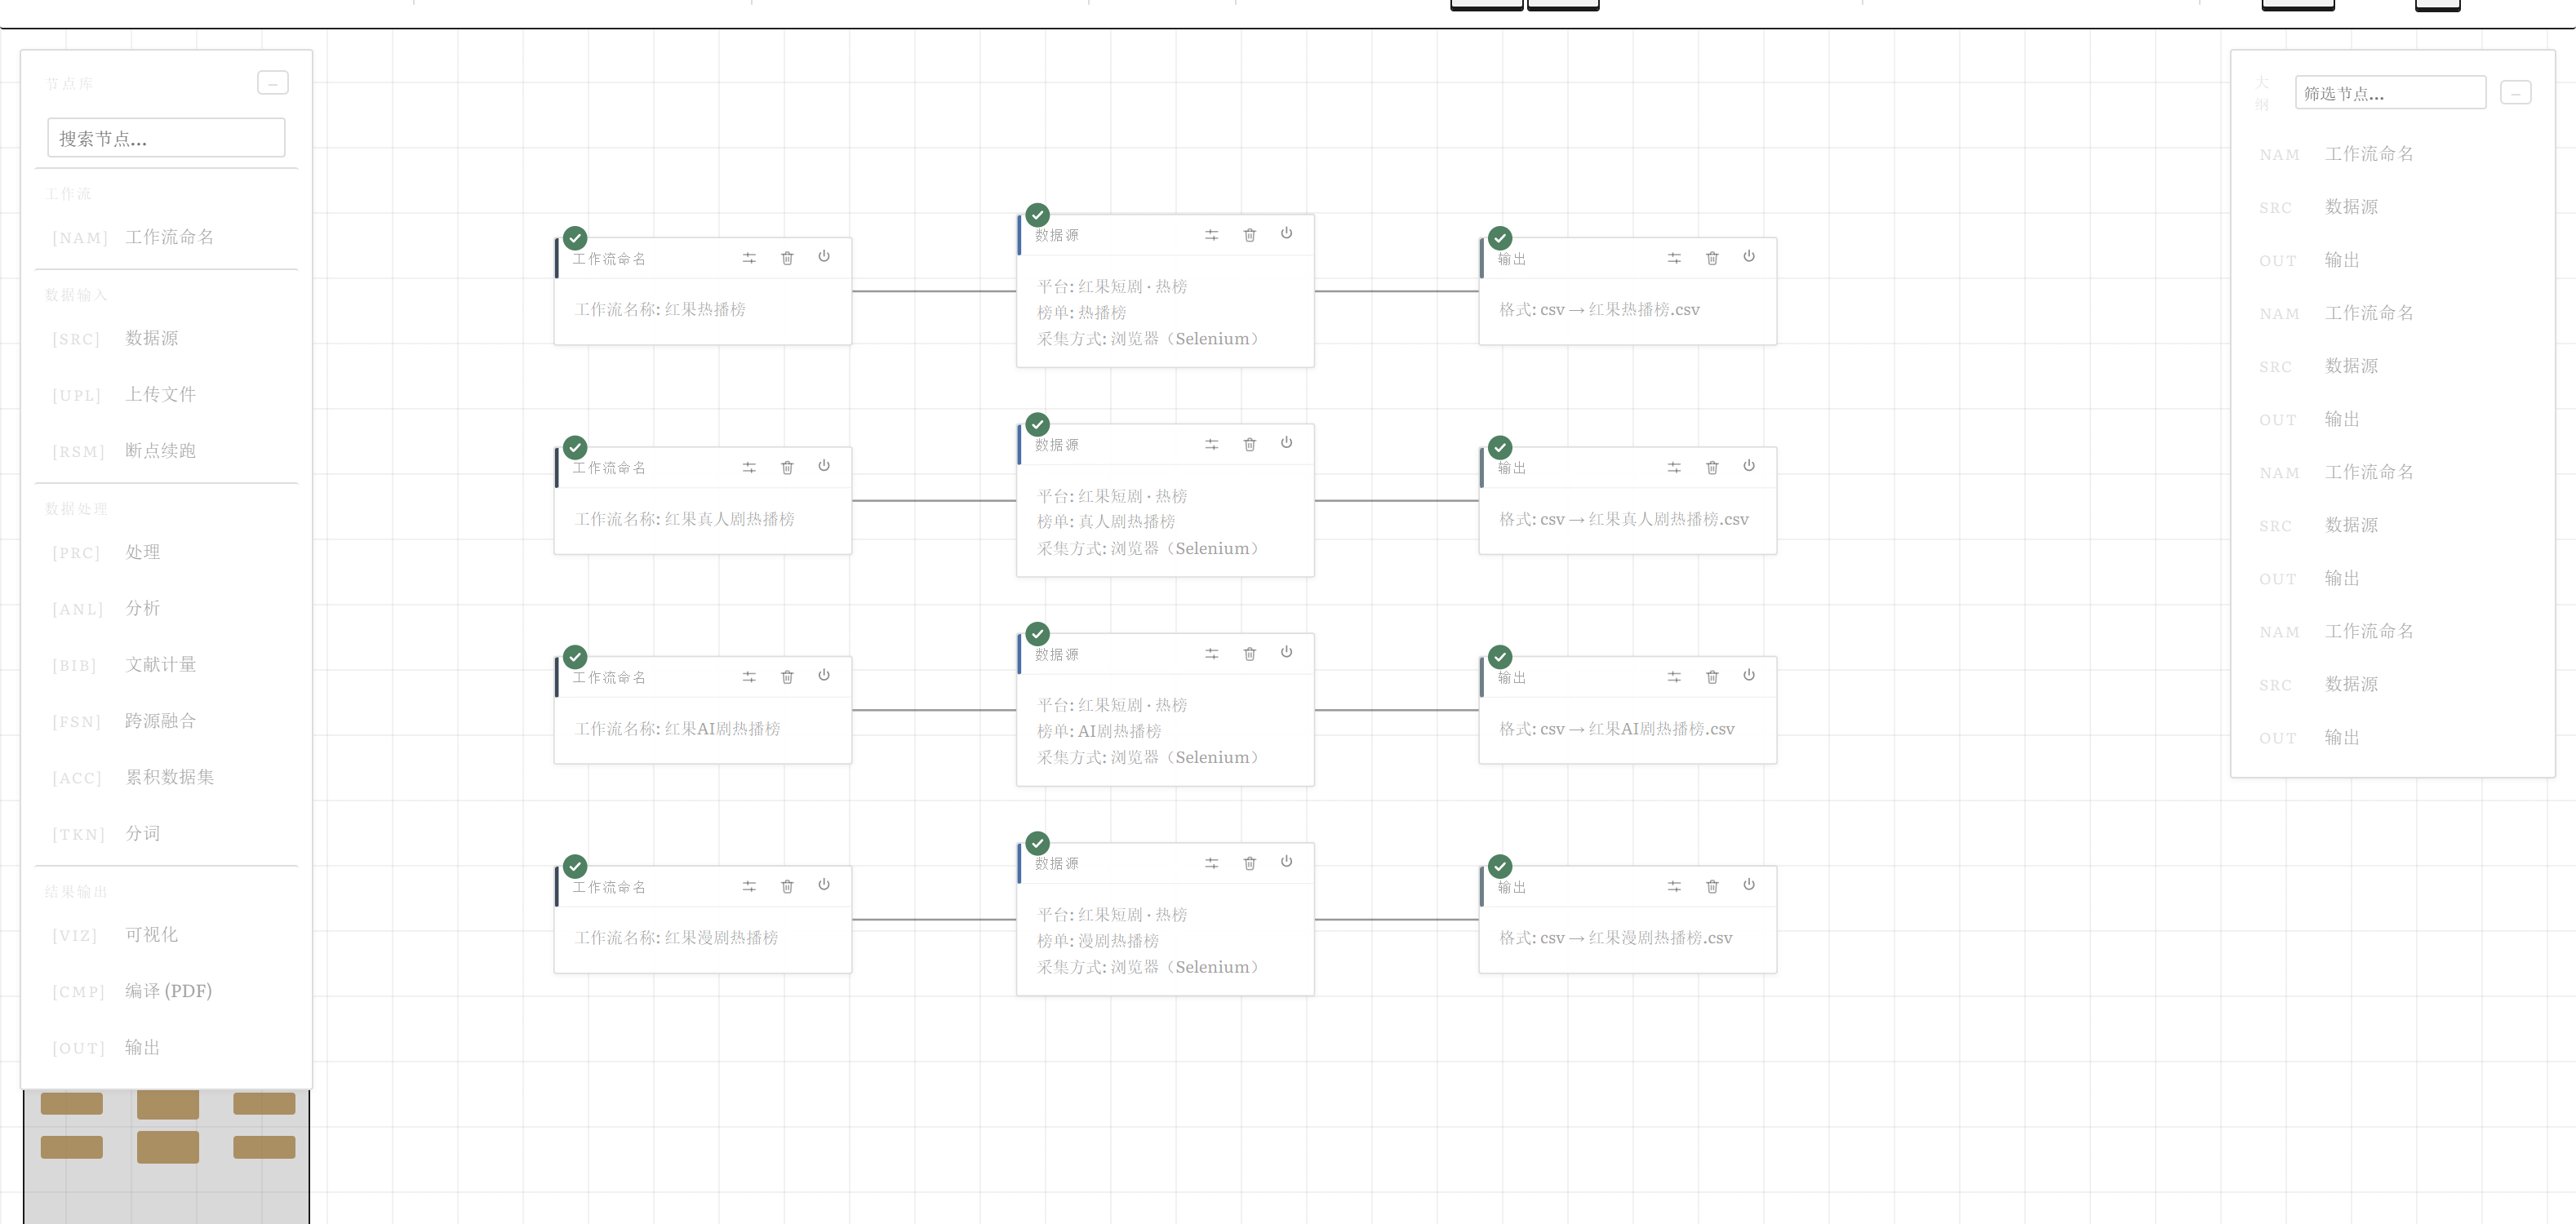
\includegraphics[width=0.98\textwidth]{hg-canvas.png}
\caption{四条链并排，可以并行跑}
\label{fig:hg-canvas}
\end{figure}

\subsection{运行}

菜单条按下“\texttt{并行}”，第一次调试可以不按“\texttt{无头}”，方便看浏览器点了哪里。点“\texttt{执行}”，
控制台先写发现四条工作流，然后四条链交错输出，每条链写每页采了多少条、累计多少、第几页是最后一页。

\begin{figure}[H]\centering
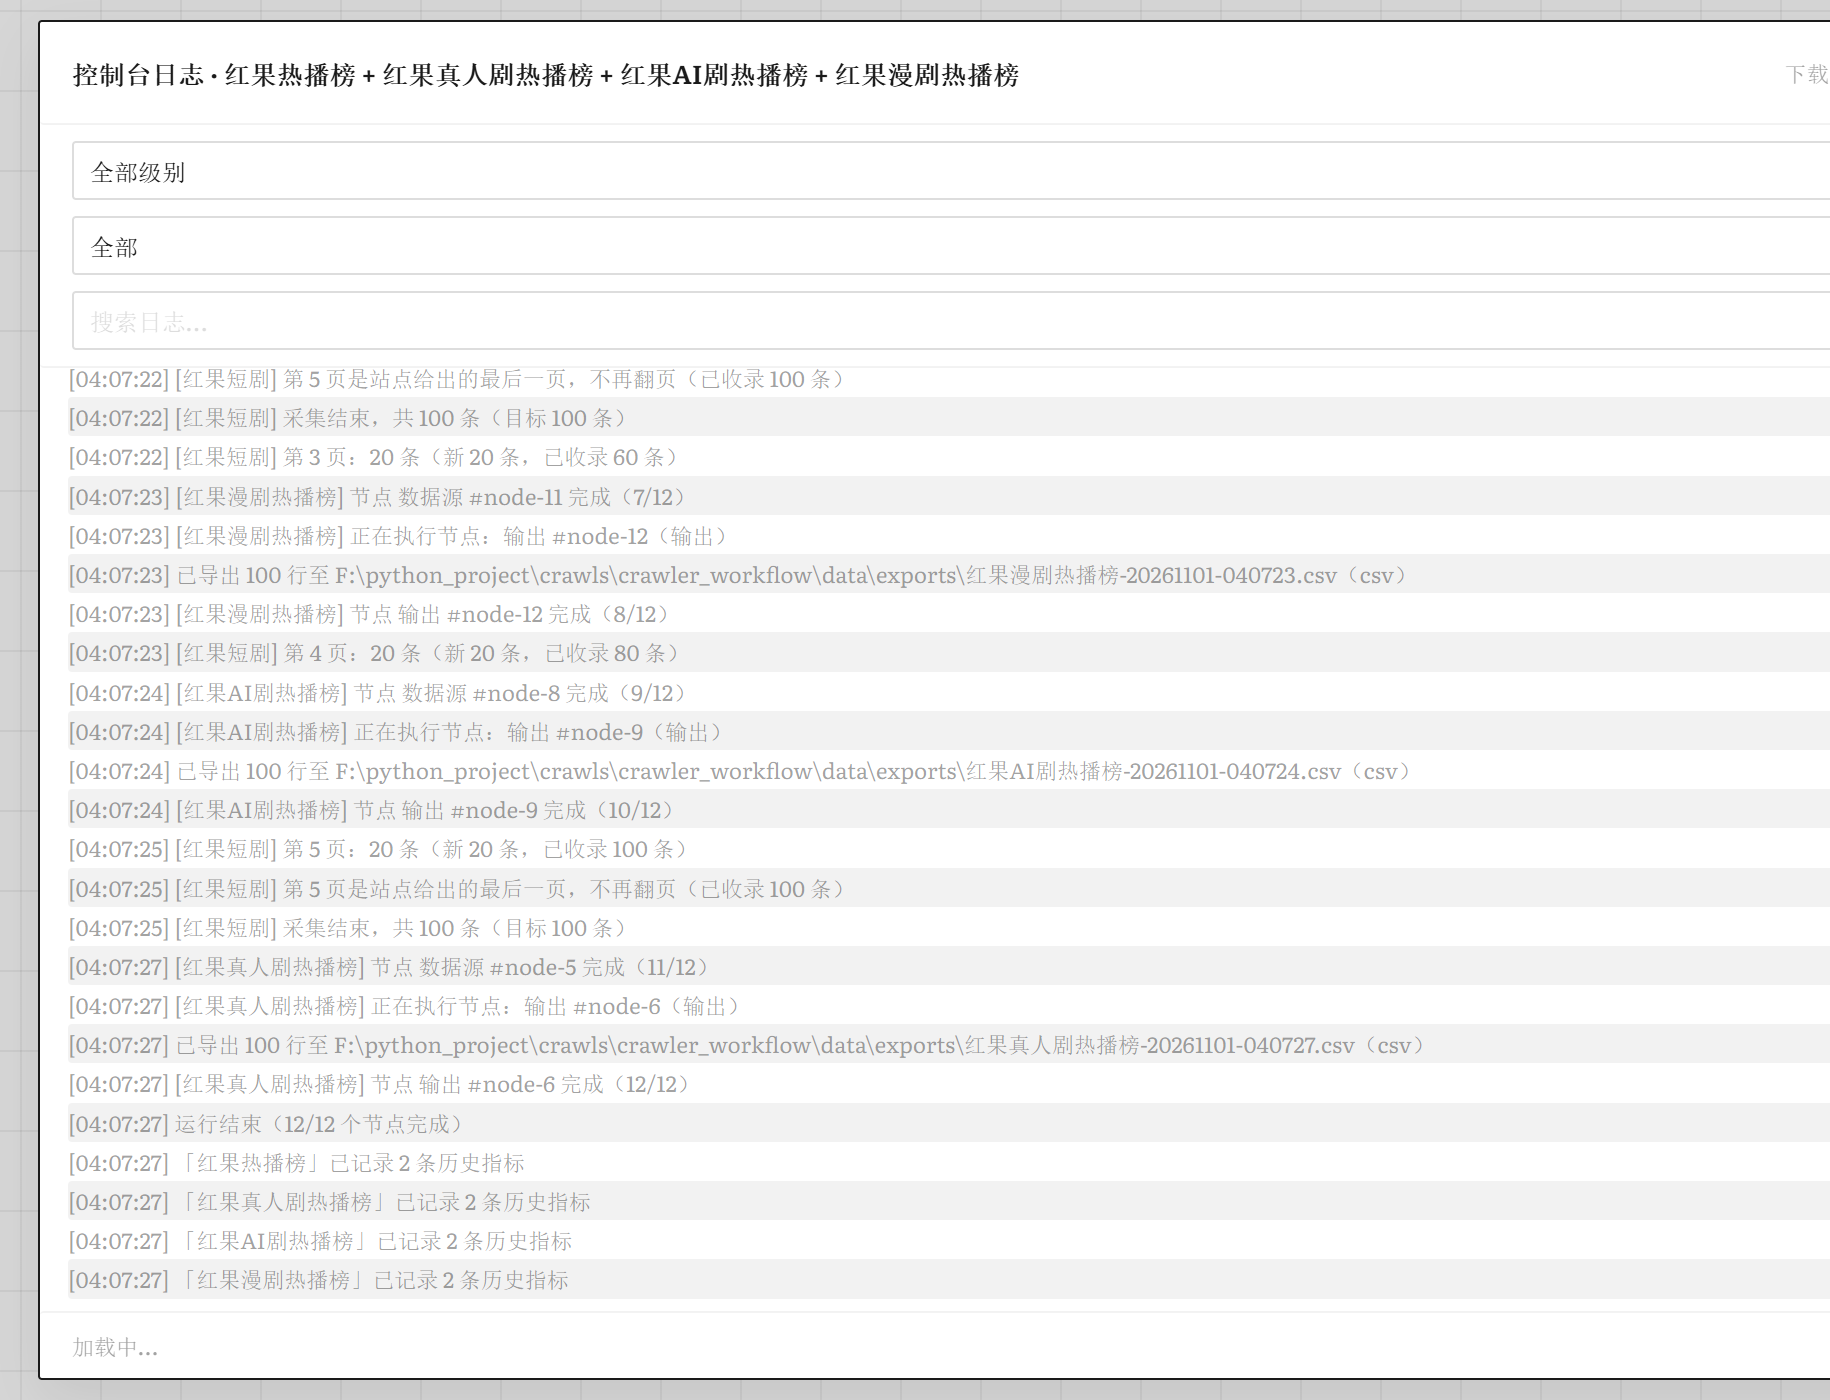
\includegraphics[width=0.94\textwidth]{run-log.png}
\caption{一次运行的完整日志，四条链交错输出}
\label{fig:hg-log}
\end{figure}

两句值得学会看：“\texttt{第 5 页是站点给出的最后一页，不再翻页（已收录 100 条）}”是站点自己的边界；
“\texttt{采集结束，共 100 条（目标 100 条）}”是这条链的结论。两句都在，就是完整结束。

\subsection{看结果}

跑完节点角标变成绿勾。数据源设置底部点“\texttt{预览数据}”，能看到这次真实落下的行：一百行十四列，
列里有作品编号、作品名、评分、热度、分类、标签。这些列名就是下游能用的列名。

\begin{figure}[H]\centering
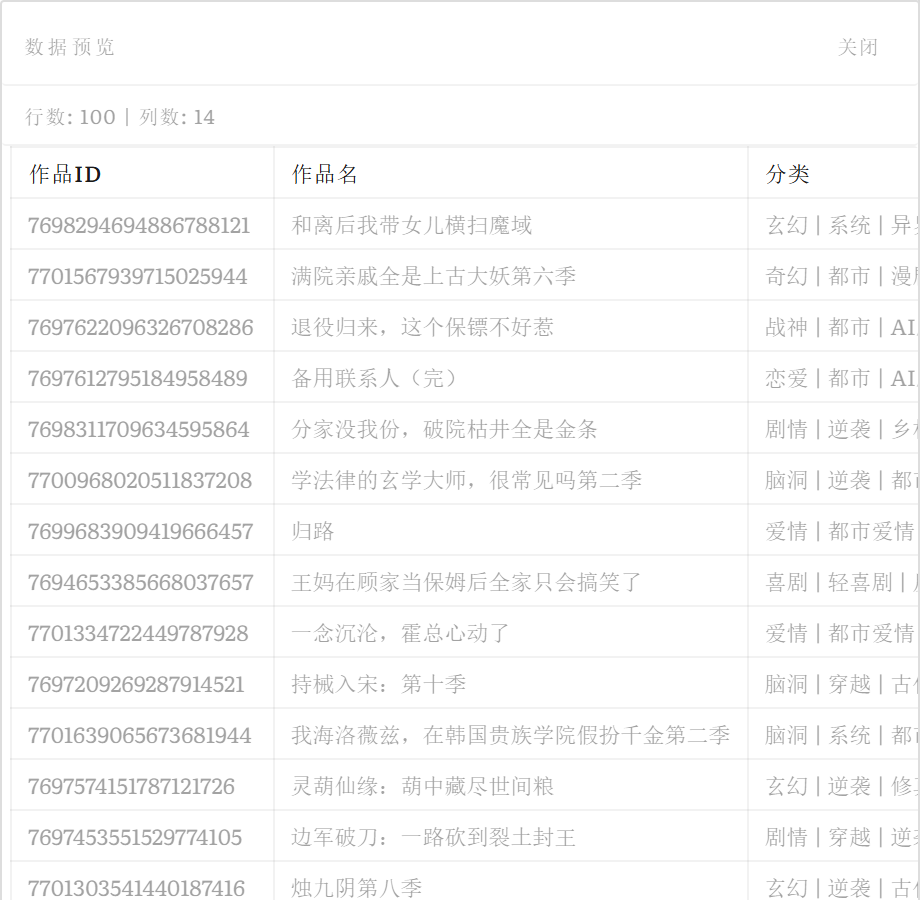
\includegraphics[width=0.9\textwidth]{hg-data.png}
\caption{预览数据：一百行十四列}
\label{fig:hg-data}
\end{figure}

底部“\texttt{导出产物}”里四份 CSV 都在，带运行时间戳，大小接近，时间挨着。点“\texttt{下载}”存到本地。

\section{实战二\quad 热榜转评论}

光有榜单没有内容。这一段把榜单当任务清单，让程序拿着每部剧的名字去抓评论。
仓库里的“\texttt{红果短剧-热榜转评论}”就是这个做法，它比上一节多一个关键动作：上游喂链接。

底部点“\texttt{工作流文件}”，找到“\texttt{红果短剧-热榜转评论}”点“\texttt{打开}”。画布上是两条链，上面一条启用，下面一条关掉。

\begin{figure}[H]\centering
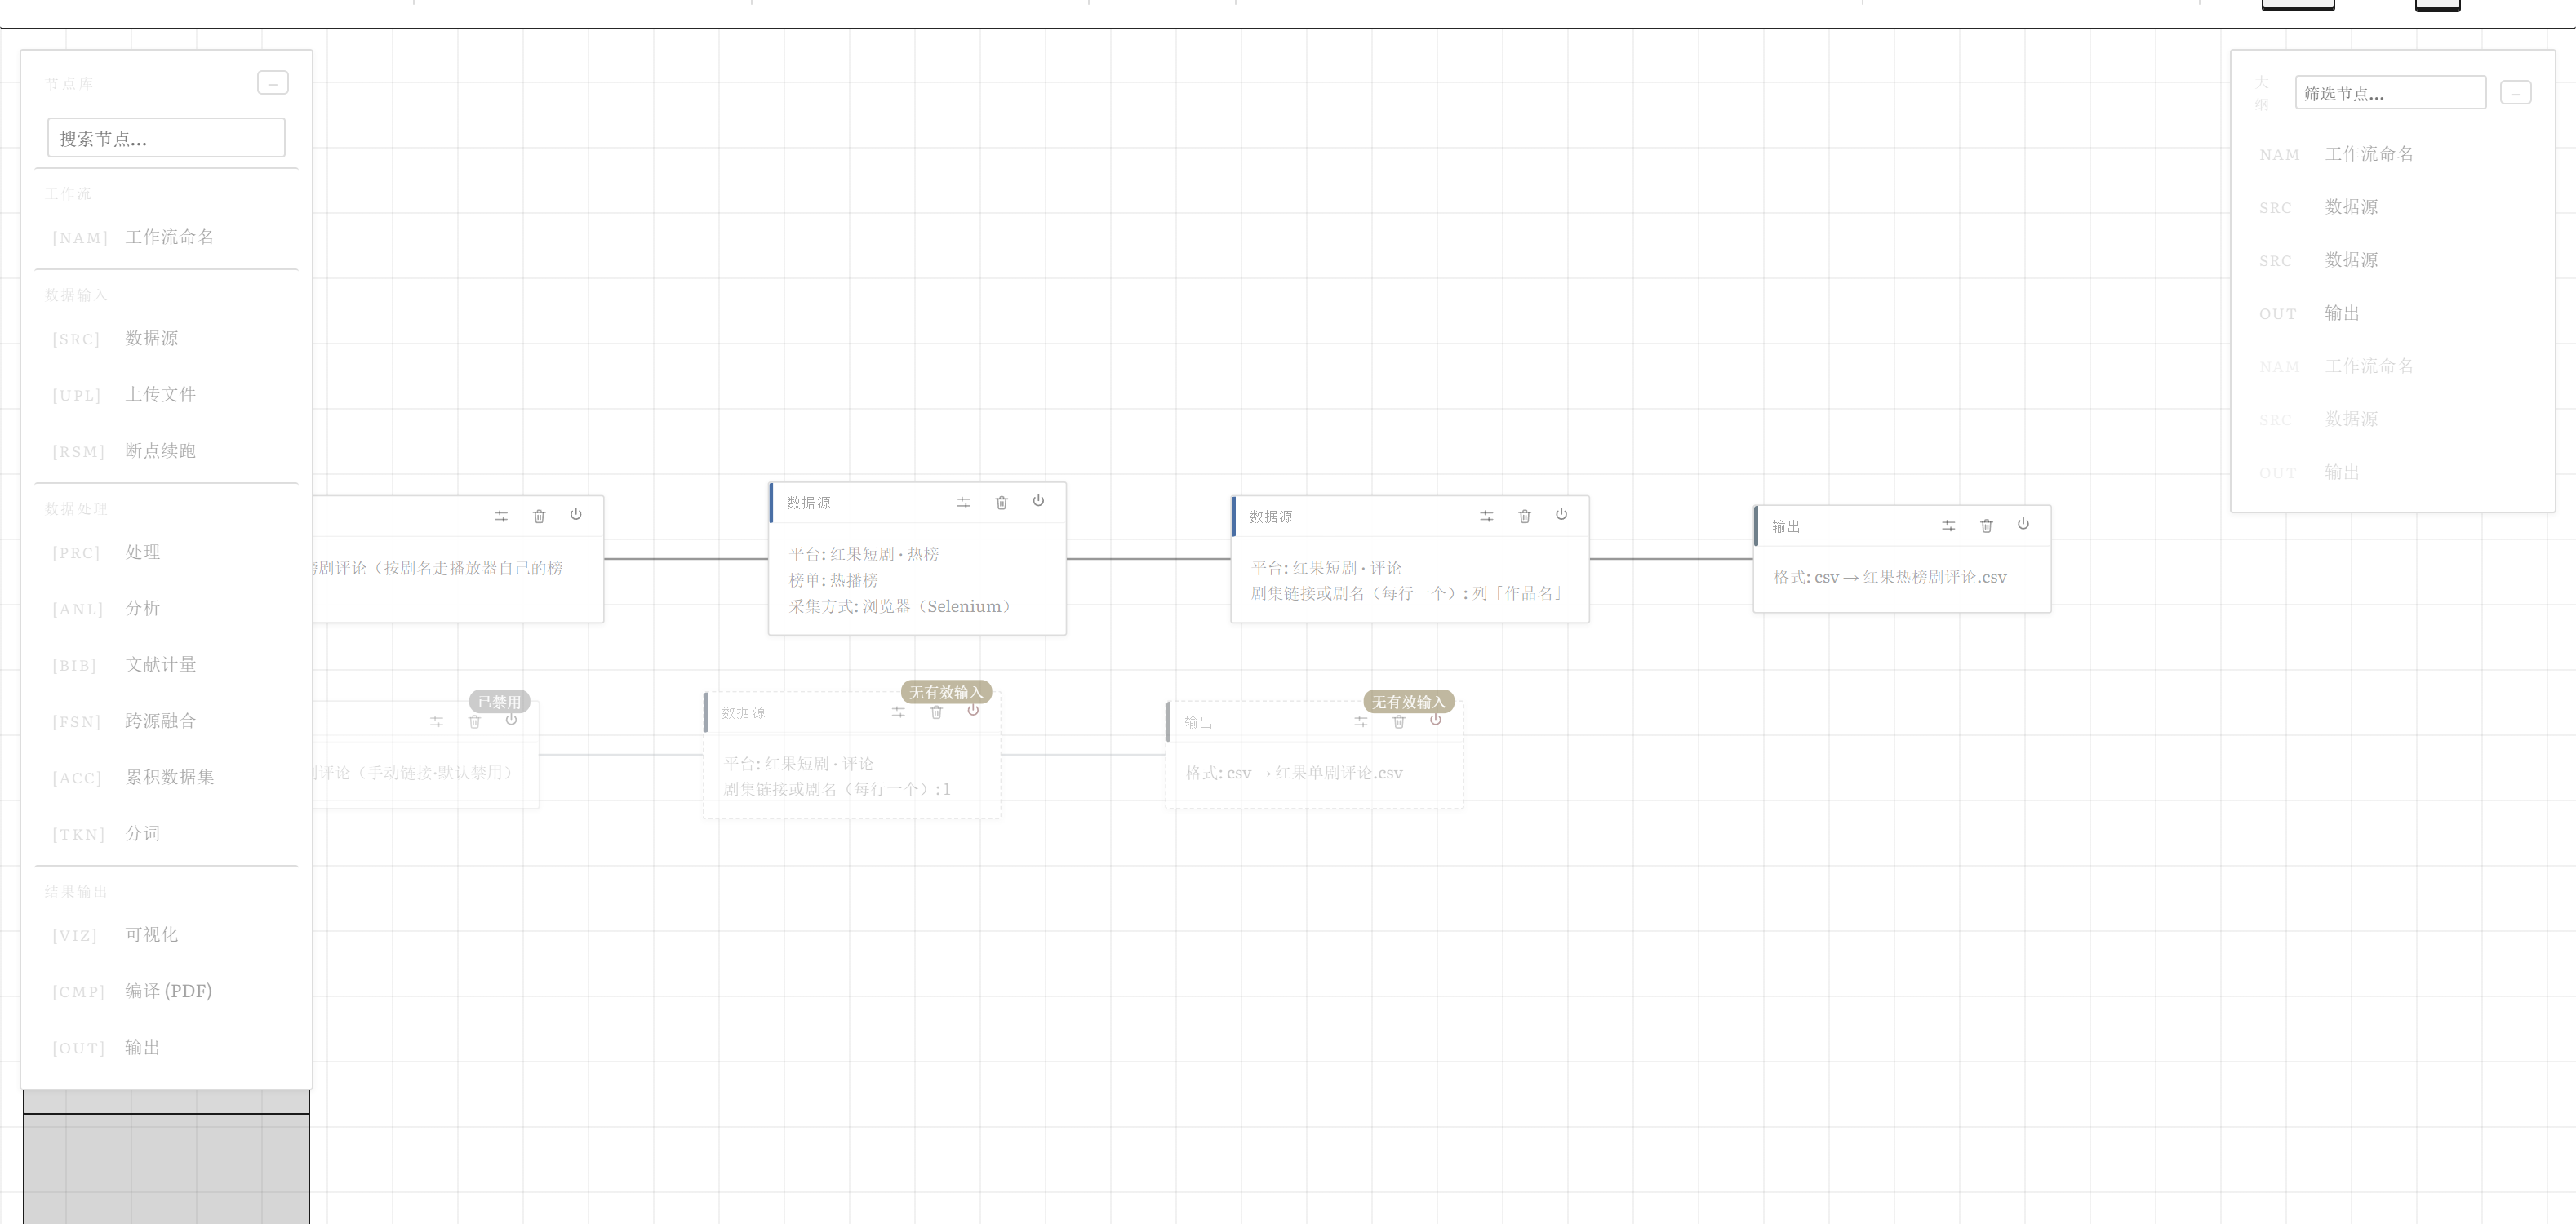
\includegraphics[width=0.98\textwidth]{hg-talk-canvas.png}
\caption{热榜转评论：上面一条启用，下面一条是手动链接的备用链}
\label{fig:hg-talk-canvas}
\end{figure}

上面第一条是命名，第二条采热播榜前十条，与实战一相同，只是数量从一百改成十。第三条才是重点：采集内容选“\texttt{评论}”，
面板里填“\texttt{每部剧集数}”5、“\texttt{包含回复}”打勾、“\texttt{收听超时}”90 秒、“\texttt{每篇单独文件}”打勾、
“\texttt{评论条数上限}”0、“\texttt{评论时间筛选}”留空，最后在“\texttt{上游列名}”填“\texttt{作品名}”。
这一栏就是上游喂任务的开关，填了它，程序逐行取这一列的片名去搜。

\begin{figure}[H]\centering

\includegraphics[width=0.31\textwidth]{hg-talk-source.png}
\caption{评论节点的上游列名填作品名，程序拿每一行的片名去搜}
\label{fig:hg-talk-source}
\end{figure}

下面那条链是手动模式，只有一个链接，写在“\texttt{文章链接}”里。命名节点被关掉，所以整条链都不跑，留着当模板：
临时想抓某一部剧，打开它换链接即可。关掉一个节点不会删掉下游，但下游会因为没有输入而一起失效，画布上是灰的，运行时真的不存在。

点执行。上面那条链先拿十条榜单，再拿每一条的剧名去驱动播放器，一条一条听，日志按剧名分组，
写听到了几集、多少条评论、存到哪个文件。红果评论不是从网页读的，程序旁听桌面播放器的通信，所以这台机器要能打开播放器。

这一节练的是两种数据流：一种从站点直接采，另一种拿上游的表当任务清单。后者可以推广到很多地方，
比如拿一份文献清单批量补摘要，拿一份博主清单批量抓主页。
